\documentclass[twoside]{book}

% Packages required by doxygen
\usepackage{fixltx2e}
\usepackage{calc}
\usepackage{doxygen}
\usepackage[export]{adjustbox} % also loads graphicx
\usepackage{graphicx}
\usepackage[utf8]{inputenc}
\usepackage{makeidx}
\usepackage{multicol}
\usepackage{multirow}
\PassOptionsToPackage{warn}{textcomp}
\usepackage{textcomp}
\usepackage[nointegrals]{wasysym}
\usepackage[table]{xcolor}

% Font selection
\usepackage[T1]{fontenc}
\usepackage[scaled=.90]{helvet}
\usepackage{courier}
\usepackage{amssymb}
\usepackage{sectsty}
\renewcommand{\familydefault}{\sfdefault}
\allsectionsfont{%
  \fontseries{bc}\selectfont%
  \color{darkgray}%
}
\renewcommand{\DoxyLabelFont}{%
  \fontseries{bc}\selectfont%
  \color{darkgray}%
}
\newcommand{\+}{\discretionary{\mbox{\scriptsize$\hookleftarrow$}}{}{}}

% Page & text layout
\usepackage{geometry}
\geometry{%
  a4paper,%
  top=2.5cm,%
  bottom=2.5cm,%
  left=2.5cm,%
  right=2.5cm%
}
\tolerance=750
\hfuzz=15pt
\hbadness=750
\setlength{\emergencystretch}{15pt}
\setlength{\parindent}{0cm}
\setlength{\parskip}{3ex plus 2ex minus 2ex}
\makeatletter
\renewcommand{\paragraph}{%
  \@startsection{paragraph}{4}{0ex}{-1.0ex}{1.0ex}{%
    \normalfont\normalsize\bfseries\SS@parafont%
  }%
}
\renewcommand{\subparagraph}{%
  \@startsection{subparagraph}{5}{0ex}{-1.0ex}{1.0ex}{%
    \normalfont\normalsize\bfseries\SS@subparafont%
  }%
}
\makeatother

% Headers & footers
\usepackage{fancyhdr}
\pagestyle{fancyplain}
\fancyhead[LE]{\fancyplain{}{\bfseries\thepage}}
\fancyhead[CE]{\fancyplain{}{}}
\fancyhead[RE]{\fancyplain{}{\bfseries\leftmark}}
\fancyhead[LO]{\fancyplain{}{\bfseries\rightmark}}
\fancyhead[CO]{\fancyplain{}{}}
\fancyhead[RO]{\fancyplain{}{\bfseries\thepage}}
\fancyfoot[LE]{\fancyplain{}{}}
\fancyfoot[CE]{\fancyplain{}{}}
\fancyfoot[RE]{\fancyplain{}{\bfseries\scriptsize Generated by Doxygen }}
\fancyfoot[LO]{\fancyplain{}{\bfseries\scriptsize Generated by Doxygen }}
\fancyfoot[CO]{\fancyplain{}{}}
\fancyfoot[RO]{\fancyplain{}{}}
\renewcommand{\footrulewidth}{0.4pt}
\renewcommand{\chaptermark}[1]{%
  \markboth{#1}{}%
}
\renewcommand{\sectionmark}[1]{%
  \markright{\thesection\ #1}%
}

% Indices & bibliography
\usepackage{natbib}
\usepackage[titles]{tocloft}
\setcounter{tocdepth}{3}
\setcounter{secnumdepth}{5}
\makeindex

% Hyperlinks (required, but should be loaded last)
\usepackage{ifpdf}
\ifpdf
  \usepackage[pdftex,pagebackref=true]{hyperref}
\else
  \usepackage[ps2pdf,pagebackref=true]{hyperref}
\fi
\hypersetup{%
  colorlinks=true,%
  linkcolor=blue,%
  citecolor=blue,%
  unicode%
}

% Custom commands
\newcommand{\clearemptydoublepage}{%
  \newpage{\pagestyle{empty}\cleardoublepage}%
}

\usepackage{caption}
\captionsetup{labelsep=space,justification=centering,font={bf},singlelinecheck=off,skip=4pt,position=top}

%===== C O N T E N T S =====

\begin{document}

% Titlepage & ToC
\hypersetup{pageanchor=false,
             bookmarksnumbered=true,
             pdfencoding=unicode
            }
\pagenumbering{roman}
\begin{titlepage}
\vspace*{7cm}
\begin{center}%
{\Large Sudoku\+Solver }\\
\vspace*{1cm}
{\large Generated by Doxygen 1.8.11}\\
\end{center}
\end{titlepage}
\clearemptydoublepage
\tableofcontents
\clearemptydoublepage
\pagenumbering{arabic}
\hypersetup{pageanchor=true}

%--- Begin generated contents ---
\chapter{Namespace Index}
\section{Namespace List}
Here is a list of all namespaces with brief descriptions\+:\begin{DoxyCompactList}
\item\contentsline{section}{\hyperlink{namespace_ui}{Ui} }{\pageref{namespace_ui}}{}
\end{DoxyCompactList}

\chapter{Hierarchical Index}
\section{Class Hierarchy}
This inheritance list is sorted roughly, but not completely, alphabetically\+:\begin{DoxyCompactList}
\item Q\+Main\+Window\begin{DoxyCompactList}
\item \contentsline{section}{Main\+Window}{\pageref{class_main_window}}{}
\end{DoxyCompactList}
\item \contentsline{section}{Sudoku\+Solver}{\pageref{class_sudoku_solver}}{}
\end{DoxyCompactList}

\chapter{Class Index}
\section{Class List}
Here are the classes, structs, unions and interfaces with brief descriptions\+:\begin{DoxyCompactList}
\item\contentsline{section}{\hyperlink{class_main_window}{Main\+Window} }{\pageref{class_main_window}}{}
\item\contentsline{section}{\hyperlink{class_sudoku_solver}{Sudoku\+Solver} \\*This method is responsible for managing the details and methods of Sudoku }{\pageref{class_sudoku_solver}}{}
\end{DoxyCompactList}

\chapter{File Index}
\section{File List}
Here is a list of all files with brief descriptions\+:\begin{DoxyCompactList}
\item\contentsline{section}{Su\+Do\+Ku\+\_\+\+Solver/\hyperlink{main_8cpp}{main.\+cpp} }{\pageref{main_8cpp}}{}
\item\contentsline{section}{Su\+Do\+Ku\+\_\+\+Solver/\hyperlink{mainwindow_8cpp}{mainwindow.\+cpp} }{\pageref{mainwindow_8cpp}}{}
\item\contentsline{section}{Su\+Do\+Ku\+\_\+\+Solver/\hyperlink{mainwindow_8h}{mainwindow.\+h} }{\pageref{mainwindow_8h}}{}
\item\contentsline{section}{Su\+Do\+Ku\+\_\+\+Solver/\hyperlink{sudokusolver_8cpp}{sudokusolver.\+cpp} }{\pageref{sudokusolver_8cpp}}{}
\item\contentsline{section}{Su\+Do\+Ku\+\_\+\+Solver/\hyperlink{sudokusolver_8h}{sudokusolver.\+h} }{\pageref{sudokusolver_8h}}{}
\end{DoxyCompactList}

\chapter{Namespace Documentation}
\hypertarget{namespace_ui}{}\section{Ui Namespace Reference}
\label{namespace_ui}\index{Ui@{Ui}}

\chapter{Class Documentation}
\hypertarget{class_main_window}{}\section{Main\+Window Class Reference}
\label{class_main_window}\index{Main\+Window@{Main\+Window}}


{\ttfamily \#include $<$mainwindow.\+h$>$}

Inheritance diagram for Main\+Window\+:\begin{figure}[H]
\begin{center}
\leavevmode
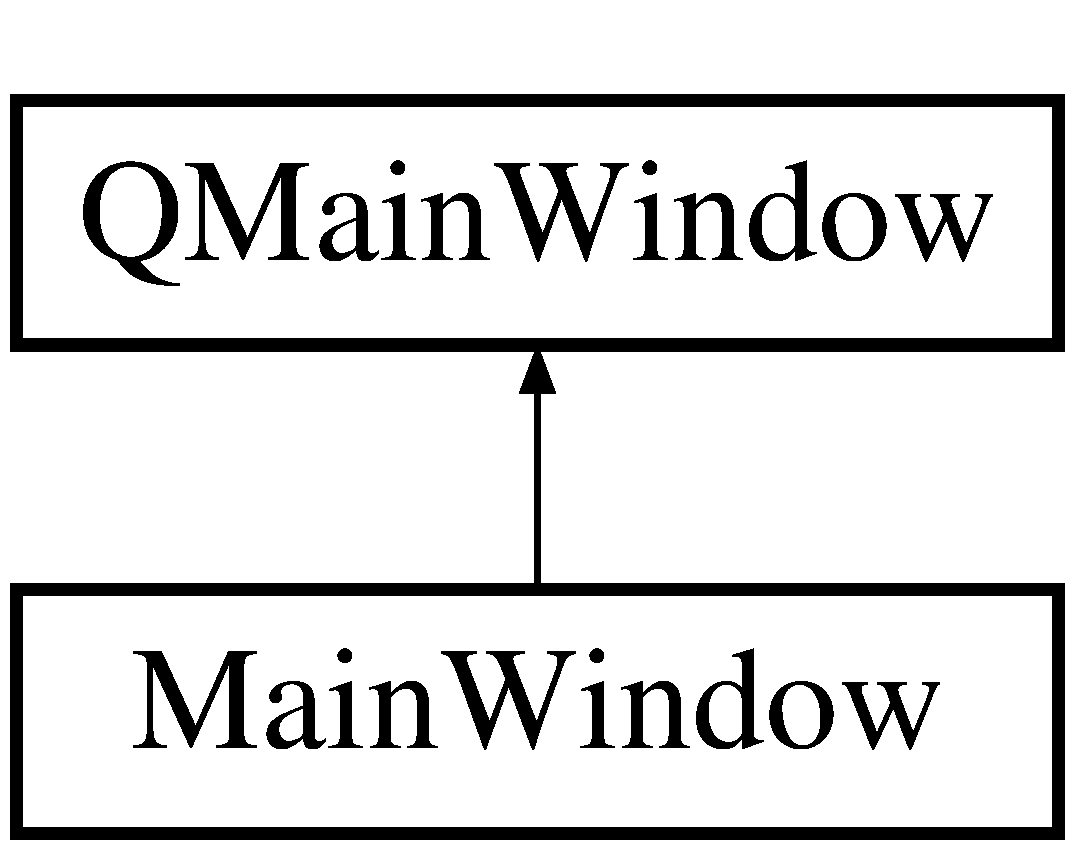
\includegraphics[height=2.000000cm]{class_main_window}
\end{center}
\end{figure}
\subsection*{Public Slots}
\begin{DoxyCompactItemize}
\item 
void \hyperlink{class_main_window_ad2301c8cd784e274020466cc90eda506}{solve\+Sudoku} ()
\item 
void \hyperlink{class_main_window_a7af642fed527fef0c6ab90a1533f5309}{clear\+Puzzle} ()
\item 
void \hyperlink{class_main_window_a90da512747ed1317b4553a04f054074a}{table\+Edit} (int row, int column)
\begin{DoxyCompactList}\small\item\em \hyperlink{class_main_window_a90da512747ed1317b4553a04f054074a}{Main\+Window\+::table\+Edit}. \end{DoxyCompactList}\item 
void \hyperlink{class_main_window_a9aa060076be05d3c231cd4df0fc74932}{change\+Mode} ()
\end{DoxyCompactItemize}
\subsection*{Public Member Functions}
\begin{DoxyCompactItemize}
\item 
\hyperlink{class_main_window_a8b244be8b7b7db1b08de2a2acb9409db}{Main\+Window} (Q\+Widget $\ast$parent=0)
\item 
\hyperlink{class_main_window_ae98d00a93bc118200eeef9f9bba1dba7}{$\sim$\+Main\+Window} ()
\end{DoxyCompactItemize}
\subsection*{Public Attributes}
\begin{DoxyCompactItemize}
\item 
\hyperlink{class_sudoku_solver}{Sudoku\+Solver} \hyperlink{class_main_window_aec079dfef291f735a37c2df4a3b46801}{solver}
\item 
bool \hyperlink{class_main_window_aa9bf5455d1599a2a9425c18de517a761}{user\+\_\+mode}
\end{DoxyCompactItemize}


\subsection{Constructor \& Destructor Documentation}
\index{Main\+Window@{Main\+Window}!Main\+Window@{Main\+Window}}
\index{Main\+Window@{Main\+Window}!Main\+Window@{Main\+Window}}
\subsubsection[{\texorpdfstring{Main\+Window(\+Q\+Widget $\ast$parent=0)}{MainWindow(QWidget *parent=0)}}]{\setlength{\rightskip}{0pt plus 5cm}Main\+Window\+::\+Main\+Window (
\begin{DoxyParamCaption}
\item[{Q\+Widget $\ast$}]{parent = {\ttfamily 0}}
\end{DoxyParamCaption}
)\hspace{0.3cm}{\ttfamily [explicit]}}\hypertarget{class_main_window_a8b244be8b7b7db1b08de2a2acb9409db}{}\label{class_main_window_a8b244be8b7b7db1b08de2a2acb9409db}
\index{Main\+Window@{Main\+Window}!````~Main\+Window@{$\sim$\+Main\+Window}}
\index{````~Main\+Window@{$\sim$\+Main\+Window}!Main\+Window@{Main\+Window}}
\subsubsection[{\texorpdfstring{$\sim$\+Main\+Window()}{~MainWindow()}}]{\setlength{\rightskip}{0pt plus 5cm}Main\+Window\+::$\sim$\+Main\+Window (
\begin{DoxyParamCaption}
{}
\end{DoxyParamCaption}
)}\hypertarget{class_main_window_ae98d00a93bc118200eeef9f9bba1dba7}{}\label{class_main_window_ae98d00a93bc118200eeef9f9bba1dba7}


\subsection{Member Function Documentation}
\index{Main\+Window@{Main\+Window}!change\+Mode@{change\+Mode}}
\index{change\+Mode@{change\+Mode}!Main\+Window@{Main\+Window}}
\subsubsection[{\texorpdfstring{change\+Mode}{changeMode}}]{\setlength{\rightskip}{0pt plus 5cm}void Main\+Window\+::change\+Mode (
\begin{DoxyParamCaption}
{}
\end{DoxyParamCaption}
)\hspace{0.3cm}{\ttfamily [slot]}}\hypertarget{class_main_window_a9aa060076be05d3c231cd4df0fc74932}{}\label{class_main_window_a9aa060076be05d3c231cd4df0fc74932}
\index{Main\+Window@{Main\+Window}!clear\+Puzzle@{clear\+Puzzle}}
\index{clear\+Puzzle@{clear\+Puzzle}!Main\+Window@{Main\+Window}}
\subsubsection[{\texorpdfstring{clear\+Puzzle}{clearPuzzle}}]{\setlength{\rightskip}{0pt plus 5cm}void Main\+Window\+::clear\+Puzzle (
\begin{DoxyParamCaption}
{}
\end{DoxyParamCaption}
)\hspace{0.3cm}{\ttfamily [slot]}}\hypertarget{class_main_window_a7af642fed527fef0c6ab90a1533f5309}{}\label{class_main_window_a7af642fed527fef0c6ab90a1533f5309}
\index{Main\+Window@{Main\+Window}!solve\+Sudoku@{solve\+Sudoku}}
\index{solve\+Sudoku@{solve\+Sudoku}!Main\+Window@{Main\+Window}}
\subsubsection[{\texorpdfstring{solve\+Sudoku}{solveSudoku}}]{\setlength{\rightskip}{0pt plus 5cm}void Main\+Window\+::solve\+Sudoku (
\begin{DoxyParamCaption}
{}
\end{DoxyParamCaption}
)\hspace{0.3cm}{\ttfamily [slot]}}\hypertarget{class_main_window_ad2301c8cd784e274020466cc90eda506}{}\label{class_main_window_ad2301c8cd784e274020466cc90eda506}
\index{Main\+Window@{Main\+Window}!table\+Edit@{table\+Edit}}
\index{table\+Edit@{table\+Edit}!Main\+Window@{Main\+Window}}
\subsubsection[{\texorpdfstring{table\+Edit}{tableEdit}}]{\setlength{\rightskip}{0pt plus 5cm}void Main\+Window\+::table\+Edit (
\begin{DoxyParamCaption}
\item[{int}]{row, }
\item[{int}]{column}
\end{DoxyParamCaption}
)\hspace{0.3cm}{\ttfamily [slot]}}\hypertarget{class_main_window_a90da512747ed1317b4553a04f054074a}{}\label{class_main_window_a90da512747ed1317b4553a04f054074a}


\hyperlink{class_main_window_a90da512747ed1317b4553a04f054074a}{Main\+Window\+::table\+Edit}. 


\begin{DoxyParams}{Parameters}
{\em row} & \\
\hline
{\em column} & This method is responsible for handling when a cell on the table is changed. \\
\hline
\end{DoxyParams}


\subsection{Member Data Documentation}
\index{Main\+Window@{Main\+Window}!solver@{solver}}
\index{solver@{solver}!Main\+Window@{Main\+Window}}
\subsubsection[{\texorpdfstring{solver}{solver}}]{\setlength{\rightskip}{0pt plus 5cm}{\bf Sudoku\+Solver} Main\+Window\+::solver}\hypertarget{class_main_window_aec079dfef291f735a37c2df4a3b46801}{}\label{class_main_window_aec079dfef291f735a37c2df4a3b46801}
\index{Main\+Window@{Main\+Window}!user\+\_\+mode@{user\+\_\+mode}}
\index{user\+\_\+mode@{user\+\_\+mode}!Main\+Window@{Main\+Window}}
\subsubsection[{\texorpdfstring{user\+\_\+mode}{user_mode}}]{\setlength{\rightskip}{0pt plus 5cm}bool Main\+Window\+::user\+\_\+mode}\hypertarget{class_main_window_aa9bf5455d1599a2a9425c18de517a761}{}\label{class_main_window_aa9bf5455d1599a2a9425c18de517a761}


The documentation for this class was generated from the following files\+:\begin{DoxyCompactItemize}
\item 
Su\+Do\+Ku\+\_\+\+Solver/\hyperlink{mainwindow_8h}{mainwindow.\+h}\item 
Su\+Do\+Ku\+\_\+\+Solver/\hyperlink{mainwindow_8cpp}{mainwindow.\+cpp}\end{DoxyCompactItemize}

\hypertarget{class_sudoku_solver}{}\section{Sudoku\+Solver Class Reference}
\label{class_sudoku_solver}\index{Sudoku\+Solver@{Sudoku\+Solver}}


The \hyperlink{class_sudoku_solver}{Sudoku\+Solver} class This method is responsible for managing the details and methods of Sudoku.  




{\ttfamily \#include $<$sudokusolver.\+h$>$}

\subsection*{Public Member Functions}
\begin{DoxyCompactItemize}
\item 
\hyperlink{class_sudoku_solver_a4bf48e09a67caff942c166ac70e42fc9}{Sudoku\+Solver} ()
\item 
bool \hyperlink{class_sudoku_solver_a14e6df202ad279fbafaf7f348f53c535}{check\+Box} (int row, int col, int test\+\_\+int)
\begin{DoxyCompactList}\small\item\em check\+Box This method tests that there are no other copies of test\+\_\+int in the 3x3 box surrounding (row,col) \end{DoxyCompactList}\item 
bool \hyperlink{class_sudoku_solver_a9312f9906262defb7ae6f4d1a56fda00}{check\+Horizontal} (int row, int col, int test\+\_\+int)
\begin{DoxyCompactList}\small\item\em check\+Horizontal This method checks that there are no instances of test\+\_\+int in the specified row, ignoring the col position \end{DoxyCompactList}\item 
bool \hyperlink{class_sudoku_solver_aecc3f72bcd6c4ba906fc20c43bd54579}{check\+Vertical} (int row, int col, int test\+\_\+int)
\begin{DoxyCompactList}\small\item\em check\+Vertical This method checks that there are no instances of test\+\_\+int in the specified column(col), ignoring the row position \end{DoxyCompactList}\item 
void \hyperlink{class_sudoku_solver_ad58cafeeb1cc40f57f37e5fac00ea40b}{set\+Input} (int row, int col, int value)
\begin{DoxyCompactList}\small\item\em set\+Input This method sets the the value at row,col for all arrays to the specified value \end{DoxyCompactList}\item 
bool \hyperlink{class_sudoku_solver_a9e2c13564d2bf647733c49cc89963553}{solve} (int row, int col)
\begin{DoxyCompactList}\small\item\em solve This method uses a recursive algorithm to solve a Sudoku problem given valid inputs \end{DoxyCompactList}\item 
void \hyperlink{class_sudoku_solver_aa86631e9684d9e5b3d77865f06323311}{reset} ()
\begin{DoxyCompactList}\small\item\em reset This method resets all arrays \end{DoxyCompactList}\item 
void \hyperlink{class_sudoku_solver_a84ba9bd3646b7357543f4499cdf4ba0f}{generate\+Puzzle} ()
\begin{DoxyCompactList}\small\item\em generate\+Puzzle This method generates a Sudoku Puzzle \end{DoxyCompactList}\item 
bool \hyperlink{class_sudoku_solver_a95305521706322fdd6d50340c6da2216}{check\+User\+Solution} ()
\begin{DoxyCompactList}\small\item\em check\+User\+Solution This method checks if the user solution is a valid solution \end{DoxyCompactList}\end{DoxyCompactItemize}
\subsection*{Public Attributes}
\begin{DoxyCompactItemize}
\item 
int \hyperlink{class_sudoku_solver_a5623374dbdea1eb6aaa857521e8ff6c2}{input} \mbox{[}9\mbox{]}\mbox{[}9\mbox{]}
\item 
int \hyperlink{class_sudoku_solver_a1aca7fe43c36b2eb07a1357f76c728d4}{solution} \mbox{[}9\mbox{]}\mbox{[}9\mbox{]}
\item 
int \hyperlink{class_sudoku_solver_a6e2f7ae7438f42979bcbd9cee385b24c}{user} \mbox{[}9\mbox{]}\mbox{[}9\mbox{]}
\end{DoxyCompactItemize}


\subsection{Detailed Description}
The \hyperlink{class_sudoku_solver}{Sudoku\+Solver} class This method is responsible for managing the details and methods of Sudoku. 

\subsection{Constructor \& Destructor Documentation}
\index{Sudoku\+Solver@{Sudoku\+Solver}!Sudoku\+Solver@{Sudoku\+Solver}}
\index{Sudoku\+Solver@{Sudoku\+Solver}!Sudoku\+Solver@{Sudoku\+Solver}}
\subsubsection[{\texorpdfstring{Sudoku\+Solver()}{SudokuSolver()}}]{\setlength{\rightskip}{0pt plus 5cm}Sudoku\+Solver\+::\+Sudoku\+Solver (
\begin{DoxyParamCaption}
{}
\end{DoxyParamCaption}
)}\hypertarget{class_sudoku_solver_a4bf48e09a67caff942c166ac70e42fc9}{}\label{class_sudoku_solver_a4bf48e09a67caff942c166ac70e42fc9}


\subsection{Member Function Documentation}
\index{Sudoku\+Solver@{Sudoku\+Solver}!check\+Box@{check\+Box}}
\index{check\+Box@{check\+Box}!Sudoku\+Solver@{Sudoku\+Solver}}
\subsubsection[{\texorpdfstring{check\+Box(int row, int col, int test\+\_\+int)}{checkBox(int row, int col, int test_int)}}]{\setlength{\rightskip}{0pt plus 5cm}bool Sudoku\+Solver\+::check\+Box (
\begin{DoxyParamCaption}
\item[{int}]{row, }
\item[{int}]{col, }
\item[{int}]{test\+\_\+int}
\end{DoxyParamCaption}
)}\hypertarget{class_sudoku_solver_a14e6df202ad279fbafaf7f348f53c535}{}\label{class_sudoku_solver_a14e6df202ad279fbafaf7f348f53c535}


check\+Box This method tests that there are no other copies of test\+\_\+int in the 3x3 box surrounding (row,col) 


\begin{DoxyParams}{Parameters}
{\em row} & \\
\hline
{\em col} & \\
\hline
{\em test\+\_\+int} & \\
\hline
\end{DoxyParams}
\begin{DoxyReturn}{Returns}
returns true if test\+\_\+int fuffils check box rules 
\end{DoxyReturn}
\index{Sudoku\+Solver@{Sudoku\+Solver}!check\+Horizontal@{check\+Horizontal}}
\index{check\+Horizontal@{check\+Horizontal}!Sudoku\+Solver@{Sudoku\+Solver}}
\subsubsection[{\texorpdfstring{check\+Horizontal(int row, int col, int test\+\_\+int)}{checkHorizontal(int row, int col, int test_int)}}]{\setlength{\rightskip}{0pt plus 5cm}bool Sudoku\+Solver\+::check\+Horizontal (
\begin{DoxyParamCaption}
\item[{int}]{row, }
\item[{int}]{col, }
\item[{int}]{test\+\_\+int}
\end{DoxyParamCaption}
)}\hypertarget{class_sudoku_solver_a9312f9906262defb7ae6f4d1a56fda00}{}\label{class_sudoku_solver_a9312f9906262defb7ae6f4d1a56fda00}


check\+Horizontal This method checks that there are no instances of test\+\_\+int in the specified row, ignoring the col position 


\begin{DoxyParams}{Parameters}
{\em row} & \\
\hline
{\em col} & \\
\hline
{\em test\+\_\+int} & \\
\hline
\end{DoxyParams}
\begin{DoxyReturn}{Returns}
returns true that test\+\_\+int satisfies the horizontal Sudoku rule 
\end{DoxyReturn}
\index{Sudoku\+Solver@{Sudoku\+Solver}!check\+User\+Solution@{check\+User\+Solution}}
\index{check\+User\+Solution@{check\+User\+Solution}!Sudoku\+Solver@{Sudoku\+Solver}}
\subsubsection[{\texorpdfstring{check\+User\+Solution()}{checkUserSolution()}}]{\setlength{\rightskip}{0pt plus 5cm}bool Sudoku\+Solver\+::check\+User\+Solution (
\begin{DoxyParamCaption}
{}
\end{DoxyParamCaption}
)}\hypertarget{class_sudoku_solver_a95305521706322fdd6d50340c6da2216}{}\label{class_sudoku_solver_a95305521706322fdd6d50340c6da2216}


check\+User\+Solution This method checks if the user solution is a valid solution 

\begin{DoxyReturn}{Returns}
returns true if the user solution is valid/correct 
\end{DoxyReturn}
\index{Sudoku\+Solver@{Sudoku\+Solver}!check\+Vertical@{check\+Vertical}}
\index{check\+Vertical@{check\+Vertical}!Sudoku\+Solver@{Sudoku\+Solver}}
\subsubsection[{\texorpdfstring{check\+Vertical(int row, int col, int test\+\_\+int)}{checkVertical(int row, int col, int test_int)}}]{\setlength{\rightskip}{0pt plus 5cm}bool Sudoku\+Solver\+::check\+Vertical (
\begin{DoxyParamCaption}
\item[{int}]{row, }
\item[{int}]{col, }
\item[{int}]{test\+\_\+int}
\end{DoxyParamCaption}
)}\hypertarget{class_sudoku_solver_aecc3f72bcd6c4ba906fc20c43bd54579}{}\label{class_sudoku_solver_aecc3f72bcd6c4ba906fc20c43bd54579}


check\+Vertical This method checks that there are no instances of test\+\_\+int in the specified column(col), ignoring the row position 


\begin{DoxyParams}{Parameters}
{\em row} & \\
\hline
{\em col} & \\
\hline
{\em test\+\_\+int} & \\
\hline
\end{DoxyParams}
\begin{DoxyReturn}{Returns}
returns true that test\+\_\+int satisfies the vertical Sudoku rule 
\end{DoxyReturn}
\index{Sudoku\+Solver@{Sudoku\+Solver}!generate\+Puzzle@{generate\+Puzzle}}
\index{generate\+Puzzle@{generate\+Puzzle}!Sudoku\+Solver@{Sudoku\+Solver}}
\subsubsection[{\texorpdfstring{generate\+Puzzle()}{generatePuzzle()}}]{\setlength{\rightskip}{0pt plus 5cm}void Sudoku\+Solver\+::generate\+Puzzle (
\begin{DoxyParamCaption}
{}
\end{DoxyParamCaption}
)}\hypertarget{class_sudoku_solver_a84ba9bd3646b7357543f4499cdf4ba0f}{}\label{class_sudoku_solver_a84ba9bd3646b7357543f4499cdf4ba0f}


generate\+Puzzle This method generates a Sudoku Puzzle 

\index{Sudoku\+Solver@{Sudoku\+Solver}!reset@{reset}}
\index{reset@{reset}!Sudoku\+Solver@{Sudoku\+Solver}}
\subsubsection[{\texorpdfstring{reset()}{reset()}}]{\setlength{\rightskip}{0pt plus 5cm}void Sudoku\+Solver\+::reset (
\begin{DoxyParamCaption}
{}
\end{DoxyParamCaption}
)}\hypertarget{class_sudoku_solver_aa86631e9684d9e5b3d77865f06323311}{}\label{class_sudoku_solver_aa86631e9684d9e5b3d77865f06323311}


reset This method resets all arrays 

\index{Sudoku\+Solver@{Sudoku\+Solver}!set\+Input@{set\+Input}}
\index{set\+Input@{set\+Input}!Sudoku\+Solver@{Sudoku\+Solver}}
\subsubsection[{\texorpdfstring{set\+Input(int row, int col, int value)}{setInput(int row, int col, int value)}}]{\setlength{\rightskip}{0pt plus 5cm}void Sudoku\+Solver\+::set\+Input (
\begin{DoxyParamCaption}
\item[{int}]{row, }
\item[{int}]{col, }
\item[{int}]{value}
\end{DoxyParamCaption}
)\hspace{0.3cm}{\ttfamily [inline]}}\hypertarget{class_sudoku_solver_ad58cafeeb1cc40f57f37e5fac00ea40b}{}\label{class_sudoku_solver_ad58cafeeb1cc40f57f37e5fac00ea40b}


set\+Input This method sets the the value at row,col for all arrays to the specified value 


\begin{DoxyParams}{Parameters}
{\em row} & \\
\hline
{\em col} & \\
\hline
{\em value} & \\
\hline
\end{DoxyParams}
\index{Sudoku\+Solver@{Sudoku\+Solver}!solve@{solve}}
\index{solve@{solve}!Sudoku\+Solver@{Sudoku\+Solver}}
\subsubsection[{\texorpdfstring{solve(int row, int col)}{solve(int row, int col)}}]{\setlength{\rightskip}{0pt plus 5cm}bool Sudoku\+Solver\+::solve (
\begin{DoxyParamCaption}
\item[{int}]{row, }
\item[{int}]{col}
\end{DoxyParamCaption}
)}\hypertarget{class_sudoku_solver_a9e2c13564d2bf647733c49cc89963553}{}\label{class_sudoku_solver_a9e2c13564d2bf647733c49cc89963553}


solve This method uses a recursive algorithm to solve a Sudoku problem given valid inputs 


\begin{DoxyParams}{Parameters}
{\em row} & \\
\hline
{\em col} & \\
\hline
\end{DoxyParams}
\begin{DoxyReturn}{Returns}
returns true if the solution is valid 
\end{DoxyReturn}


\subsection{Member Data Documentation}
\index{Sudoku\+Solver@{Sudoku\+Solver}!input@{input}}
\index{input@{input}!Sudoku\+Solver@{Sudoku\+Solver}}
\subsubsection[{\texorpdfstring{input}{input}}]{\setlength{\rightskip}{0pt plus 5cm}int Sudoku\+Solver\+::input\mbox{[}9\mbox{]}\mbox{[}9\mbox{]}}\hypertarget{class_sudoku_solver_a5623374dbdea1eb6aaa857521e8ff6c2}{}\label{class_sudoku_solver_a5623374dbdea1eb6aaa857521e8ff6c2}
\index{Sudoku\+Solver@{Sudoku\+Solver}!solution@{solution}}
\index{solution@{solution}!Sudoku\+Solver@{Sudoku\+Solver}}
\subsubsection[{\texorpdfstring{solution}{solution}}]{\setlength{\rightskip}{0pt plus 5cm}int Sudoku\+Solver\+::solution\mbox{[}9\mbox{]}\mbox{[}9\mbox{]}}\hypertarget{class_sudoku_solver_a1aca7fe43c36b2eb07a1357f76c728d4}{}\label{class_sudoku_solver_a1aca7fe43c36b2eb07a1357f76c728d4}
\index{Sudoku\+Solver@{Sudoku\+Solver}!user@{user}}
\index{user@{user}!Sudoku\+Solver@{Sudoku\+Solver}}
\subsubsection[{\texorpdfstring{user}{user}}]{\setlength{\rightskip}{0pt plus 5cm}int Sudoku\+Solver\+::user\mbox{[}9\mbox{]}\mbox{[}9\mbox{]}}\hypertarget{class_sudoku_solver_a6e2f7ae7438f42979bcbd9cee385b24c}{}\label{class_sudoku_solver_a6e2f7ae7438f42979bcbd9cee385b24c}


The documentation for this class was generated from the following files\+:\begin{DoxyCompactItemize}
\item 
Su\+Do\+Ku\+\_\+\+Solver/\hyperlink{sudokusolver_8h}{sudokusolver.\+h}\item 
Su\+Do\+Ku\+\_\+\+Solver/\hyperlink{sudokusolver_8cpp}{sudokusolver.\+cpp}\end{DoxyCompactItemize}

\chapter{File Documentation}
\hypertarget{main_8cpp}{}\section{Su\+Do\+Ku\+\_\+\+Solver/main.cpp File Reference}
\label{main_8cpp}\index{Su\+Do\+Ku\+\_\+\+Solver/main.\+cpp@{Su\+Do\+Ku\+\_\+\+Solver/main.\+cpp}}
{\ttfamily \#include \char`\"{}mainwindow.\+h\char`\"{}}\\*
{\ttfamily \#include $<$Q\+Application$>$}\\*
\subsection*{Functions}
\begin{DoxyCompactItemize}
\item 
int \hyperlink{main_8cpp_a0ddf1224851353fc92bfbff6f499fa97}{main} (int argc, char $\ast$argv\mbox{[}$\,$\mbox{]})
\end{DoxyCompactItemize}


\subsection{Function Documentation}
\index{main.\+cpp@{main.\+cpp}!main@{main}}
\index{main@{main}!main.\+cpp@{main.\+cpp}}
\subsubsection[{\texorpdfstring{main(int argc, char $\ast$argv[])}{main(int argc, char *argv[])}}]{\setlength{\rightskip}{0pt plus 5cm}int main (
\begin{DoxyParamCaption}
\item[{int}]{argc, }
\item[{char $\ast$}]{argv\mbox{[}$\,$\mbox{]}}
\end{DoxyParamCaption}
)}\hypertarget{main_8cpp_a0ddf1224851353fc92bfbff6f499fa97}{}\label{main_8cpp_a0ddf1224851353fc92bfbff6f499fa97}

\hypertarget{mainwindow_8cpp}{}\section{Su\+Do\+Ku\+\_\+\+Solver/mainwindow.cpp File Reference}
\label{mainwindow_8cpp}\index{Su\+Do\+Ku\+\_\+\+Solver/mainwindow.\+cpp@{Su\+Do\+Ku\+\_\+\+Solver/mainwindow.\+cpp}}
{\ttfamily \#include \char`\"{}mainwindow.\+h\char`\"{}}\\*
{\ttfamily \#include \char`\"{}ui\+\_\+mainwindow.\+h\char`\"{}}\\*
{\ttfamily \#include $<$iostream$>$}\\*

\hypertarget{mainwindow_8h}{}\section{Su\+Do\+Ku\+\_\+\+Solver/mainwindow.h File Reference}
\label{mainwindow_8h}\index{Su\+Do\+Ku\+\_\+\+Solver/mainwindow.\+h@{Su\+Do\+Ku\+\_\+\+Solver/mainwindow.\+h}}
{\ttfamily \#include $<$Q\+Main\+Window$>$}\\*
{\ttfamily \#include $<$ui\+\_\+mainwindow.\+h$>$}\\*
{\ttfamily \#include $<$sudokusolver.\+h$>$}\\*
\subsection*{Classes}
\begin{DoxyCompactItemize}
\item 
class \hyperlink{class_main_window}{Main\+Window}
\end{DoxyCompactItemize}
\subsection*{Namespaces}
\begin{DoxyCompactItemize}
\item 
 \hyperlink{namespace_ui}{Ui}
\end{DoxyCompactItemize}

\hypertarget{sudokusolver_8cpp}{}\section{Su\+Do\+Ku\+\_\+\+Solver/sudokusolver.cpp File Reference}
\label{sudokusolver_8cpp}\index{Su\+Do\+Ku\+\_\+\+Solver/sudokusolver.\+cpp@{Su\+Do\+Ku\+\_\+\+Solver/sudokusolver.\+cpp}}
{\ttfamily \#include \char`\"{}sudokusolver.\+h\char`\"{}}\\*
{\ttfamily \#include $<$iostream$>$}\\*

\hypertarget{sudokusolver_8h}{}\section{Su\+Do\+Ku\+\_\+\+Solver/sudokusolver.h File Reference}
\label{sudokusolver_8h}\index{Su\+Do\+Ku\+\_\+\+Solver/sudokusolver.\+h@{Su\+Do\+Ku\+\_\+\+Solver/sudokusolver.\+h}}
\subsection*{Classes}
\begin{DoxyCompactItemize}
\item 
class \hyperlink{class_sudoku_solver}{Sudoku\+Solver}
\begin{DoxyCompactList}\small\item\em The \hyperlink{class_sudoku_solver}{Sudoku\+Solver} class This method is responsible for managing the details and methods of Sudoku. \end{DoxyCompactList}\end{DoxyCompactItemize}

%--- End generated contents ---

% Index
\backmatter
\newpage
\phantomsection
\clearemptydoublepage
\addcontentsline{toc}{chapter}{Index}
\printindex

\end{document}
